% Options for packages loaded elsewhere
\PassOptionsToPackage{unicode}{hyperref}
\PassOptionsToPackage{hyphens}{url}
%
\documentclass[
]{article}
\usepackage{amsmath,amssymb}
\usepackage{iftex}
\ifPDFTeX
  \usepackage[T1]{fontenc}
  \usepackage[utf8]{inputenc}
  \usepackage{textcomp} % provide euro and other symbols
\else % if luatex or xetex
  \usepackage{unicode-math} % this also loads fontspec
  \defaultfontfeatures{Scale=MatchLowercase}
  \defaultfontfeatures[\rmfamily]{Ligatures=TeX,Scale=1}
\fi
\usepackage{lmodern}
\ifPDFTeX\else
  % xetex/luatex font selection
\fi
% Use upquote if available, for straight quotes in verbatim environments
\IfFileExists{upquote.sty}{\usepackage{upquote}}{}
\IfFileExists{microtype.sty}{% use microtype if available
  \usepackage[]{microtype}
  \UseMicrotypeSet[protrusion]{basicmath} % disable protrusion for tt fonts
}{}
\makeatletter
\@ifundefined{KOMAClassName}{% if non-KOMA class
  \IfFileExists{parskip.sty}{%
    \usepackage{parskip}
  }{% else
    \setlength{\parindent}{0pt}
    \setlength{\parskip}{6pt plus 2pt minus 1pt}}
}{% if KOMA class
  \KOMAoptions{parskip=half}}
\makeatother
\usepackage{xcolor}
\usepackage[margin=1in]{geometry}
\usepackage{color}
\usepackage{fancyvrb}
\newcommand{\VerbBar}{|}
\newcommand{\VERB}{\Verb[commandchars=\\\{\}]}
\DefineVerbatimEnvironment{Highlighting}{Verbatim}{commandchars=\\\{\}}
% Add ',fontsize=\small' for more characters per line
\usepackage{framed}
\definecolor{shadecolor}{RGB}{248,248,248}
\newenvironment{Shaded}{\begin{snugshade}}{\end{snugshade}}
\newcommand{\AlertTok}[1]{\textcolor[rgb]{0.94,0.16,0.16}{#1}}
\newcommand{\AnnotationTok}[1]{\textcolor[rgb]{0.56,0.35,0.01}{\textbf{\textit{#1}}}}
\newcommand{\AttributeTok}[1]{\textcolor[rgb]{0.13,0.29,0.53}{#1}}
\newcommand{\BaseNTok}[1]{\textcolor[rgb]{0.00,0.00,0.81}{#1}}
\newcommand{\BuiltInTok}[1]{#1}
\newcommand{\CharTok}[1]{\textcolor[rgb]{0.31,0.60,0.02}{#1}}
\newcommand{\CommentTok}[1]{\textcolor[rgb]{0.56,0.35,0.01}{\textit{#1}}}
\newcommand{\CommentVarTok}[1]{\textcolor[rgb]{0.56,0.35,0.01}{\textbf{\textit{#1}}}}
\newcommand{\ConstantTok}[1]{\textcolor[rgb]{0.56,0.35,0.01}{#1}}
\newcommand{\ControlFlowTok}[1]{\textcolor[rgb]{0.13,0.29,0.53}{\textbf{#1}}}
\newcommand{\DataTypeTok}[1]{\textcolor[rgb]{0.13,0.29,0.53}{#1}}
\newcommand{\DecValTok}[1]{\textcolor[rgb]{0.00,0.00,0.81}{#1}}
\newcommand{\DocumentationTok}[1]{\textcolor[rgb]{0.56,0.35,0.01}{\textbf{\textit{#1}}}}
\newcommand{\ErrorTok}[1]{\textcolor[rgb]{0.64,0.00,0.00}{\textbf{#1}}}
\newcommand{\ExtensionTok}[1]{#1}
\newcommand{\FloatTok}[1]{\textcolor[rgb]{0.00,0.00,0.81}{#1}}
\newcommand{\FunctionTok}[1]{\textcolor[rgb]{0.13,0.29,0.53}{\textbf{#1}}}
\newcommand{\ImportTok}[1]{#1}
\newcommand{\InformationTok}[1]{\textcolor[rgb]{0.56,0.35,0.01}{\textbf{\textit{#1}}}}
\newcommand{\KeywordTok}[1]{\textcolor[rgb]{0.13,0.29,0.53}{\textbf{#1}}}
\newcommand{\NormalTok}[1]{#1}
\newcommand{\OperatorTok}[1]{\textcolor[rgb]{0.81,0.36,0.00}{\textbf{#1}}}
\newcommand{\OtherTok}[1]{\textcolor[rgb]{0.56,0.35,0.01}{#1}}
\newcommand{\PreprocessorTok}[1]{\textcolor[rgb]{0.56,0.35,0.01}{\textit{#1}}}
\newcommand{\RegionMarkerTok}[1]{#1}
\newcommand{\SpecialCharTok}[1]{\textcolor[rgb]{0.81,0.36,0.00}{\textbf{#1}}}
\newcommand{\SpecialStringTok}[1]{\textcolor[rgb]{0.31,0.60,0.02}{#1}}
\newcommand{\StringTok}[1]{\textcolor[rgb]{0.31,0.60,0.02}{#1}}
\newcommand{\VariableTok}[1]{\textcolor[rgb]{0.00,0.00,0.00}{#1}}
\newcommand{\VerbatimStringTok}[1]{\textcolor[rgb]{0.31,0.60,0.02}{#1}}
\newcommand{\WarningTok}[1]{\textcolor[rgb]{0.56,0.35,0.01}{\textbf{\textit{#1}}}}
\usepackage{graphicx}
\makeatletter
\newsavebox\pandoc@box
\newcommand*\pandocbounded[1]{% scales image to fit in text height/width
  \sbox\pandoc@box{#1}%
  \Gscale@div\@tempa{\textheight}{\dimexpr\ht\pandoc@box+\dp\pandoc@box\relax}%
  \Gscale@div\@tempb{\linewidth}{\wd\pandoc@box}%
  \ifdim\@tempb\p@<\@tempa\p@\let\@tempa\@tempb\fi% select the smaller of both
  \ifdim\@tempa\p@<\p@\scalebox{\@tempa}{\usebox\pandoc@box}%
  \else\usebox{\pandoc@box}%
  \fi%
}
% Set default figure placement to htbp
\def\fps@figure{htbp}
\makeatother
\setlength{\emergencystretch}{3em} % prevent overfull lines
\providecommand{\tightlist}{%
  \setlength{\itemsep}{0pt}\setlength{\parskip}{0pt}}
\setcounter{secnumdepth}{-\maxdimen} % remove section numbering
\usepackage{bookmark}
\IfFileExists{xurl.sty}{\usepackage{xurl}}{} % add URL line breaks if available
\urlstyle{same}
\hypersetup{
  pdftitle={Data Cleaning: Eurovision},
  pdfauthor={Max Glonek},
  hidelinks,
  pdfcreator={LaTeX via pandoc}}

\title{Data Cleaning: Eurovision}
\author{Max Glonek}
\date{Trimester 1, 2025}

\begin{document}
\maketitle

{
\setcounter{tocdepth}{2}
\tableofcontents
}
\section{Rule 1: Look at the Data}\label{rule-1-look-at-the-data}

\section{Rule 2: Is There a Package to Deal With
That}\label{rule-2-is-there-a-package-to-deal-with-that}

\begin{Shaded}
\begin{Highlighting}[]
\NormalTok{songs }\OtherTok{\textless{}{-}}\NormalTok{ jsonlite}\SpecialCharTok{::}\FunctionTok{fromJSON}\NormalTok{(glue}\SpecialCharTok{::}\FunctionTok{glue}\NormalTok{(}\StringTok{"./data/eurovision{-}lyrics.json"}\NormalTok{))}
\end{Highlighting}
\end{Shaded}

\section{Rule 3: Break it Into
Pieces}\label{rule-3-break-it-into-pieces}

\begin{Shaded}
\begin{Highlighting}[]
\NormalTok{songs[[}\DecValTok{1}\NormalTok{]]}
\end{Highlighting}
\end{Shaded}

\begin{verbatim}
## $`#`
## [1] "1"
## 
## $Country
## [1] "Netherlands"
## 
## $`#.1`
## [1] "1"
## 
## $Artist
## [1] "Jetty Paerl"
## 
## $Song
## [1] "De vogels van Holland"
## 
## $Language
## [1] "Dutch"
## 
## $Pl.
## [1] "-"
## 
## $Sc.
## [1] "-"
## 
## $Eurovision_Number
## [1] 1
## 
## $Year
## [1] "1956"
## 
## $Host_Country
## [1] "Switzerland"
## 
## $Host_City
## [1] "Lugano"
## 
## $Lyrics
## [1] "De vogels van Holland zijn zo muzikaal\nZe leren in hun prille jeugd al tierelieren\nDe merel, de lijster en de nachtegaal\nOm zo de lente in Holland goed te kunnen vieren\n\nHet is geen wonder, want nergens\nZijn de plassen zo blauw\nAls in Holland - mijnheer\nAls in Holland - mevrouw\nHet is geen wonder, want nergens\nIs het gras zo vol dauw\nZijn de meisjes zo lief\nZijn de meisjes zo trouw\nEn daarom zijn de vogels hier allemaal\nZo muzikaal, zo muzikaal, zo muzikaal\n\nDe hele wereld door heb ik vogels horen zingen\nIn het zuiden, in het westen, in het noorden\nIn vele verre landen heb ik vogels horen zingen\nZij zingen kleine liedjes zonder woorden\n\nDe Franse vogels zingen \"tudeludelu\"\nJapanse vogels zingen \"tudeludelu\"\nChinese vogels zingen \"tudeludelu\"\nMaar de vogels zingen nergens\nZo gelukkig en blij\nAls in Holland in het voorjaar in de wei\n\nDe vogels van Holland zijn zo muzikaal\nZe leren in hun prille jeugd al tierelieren\nDe merel, de lijster en de nachtegaal\nOm zo de lente in Holland goed te kunnen vieren\n\nHet is geen wonder, want nergens\nZijn de plassen zo blauw\nAls in Holland - mijnheer\nAls in Holland - mevrouw\nHet is geen wonder, want nergens\nIs het gras zo vol dauw\nZijn de meisjes zo lief\nZijn de meisjes zo trouw\nEn daarom zijn de vogels hier allemaal\nZo muzikaal, zo muzikaal, zo muzikaal"
## 
## $`Lyrics translation`
## [1] "The birds of Holland are so musical\nThey already learn to twitter in their early youth\nThe blackbird, the thrush and the nightingale\nSo they can celebrate spring in Holland It's no wonder, because nowhere the puddles are so blue\nAs in Holland, sir\nAs in Holland, madam\nIt's no wonder, because nowhere the grass is so full of dew Are the girls so sweet, are the girls so faithfull\nAnd that's why all the birds here are\nSo musical, So musical, So musical Across the whole world I've heard birds sing\nTo the south, to the west, to the north\nIn many faraway countries I've heard birds sing\nThey sing little songs without words The French birds sing toodledoo\nJapanese birds sing toodledoo\nChinese birds sing toodledoo\nBut nowhere the birds sing so happily and cheerfully\nAs in Holland in spring in the meadow The birds of Holland are so musical\nThey already learn to twitter in their early youth\nThe blackbird, the thrush and the nightingale\nSo they can celebrate the spring in Holland It's no wonder, because nowhere the puddles are so blue\n As in Holland, sir\n As in Holland, madam\nIt's no wonder, because nowhere the grass is so full of dew Are the girls so sweet, are the girls so faithfull\nAnd that's why all the birds here are\nSo musical, So musical, So musical"
\end{verbatim}

\begin{Shaded}
\begin{Highlighting}[]
\NormalTok{parse\_song }\OtherTok{\textless{}{-}} \ControlFlowTok{function}\NormalTok{(song)\{}
\NormalTok{  country }\OtherTok{\textless{}{-}}\NormalTok{ song}\SpecialCharTok{$}\NormalTok{Country}
\NormalTok{  artist }\OtherTok{\textless{}{-}}\NormalTok{ song}\SpecialCharTok{$}\NormalTok{Artist}
\NormalTok{  title }\OtherTok{\textless{}{-}}\NormalTok{ song}\SpecialCharTok{$}\NormalTok{Song}
\NormalTok{  year }\OtherTok{\textless{}{-}}\NormalTok{ song}\SpecialCharTok{$}\NormalTok{Year}
\NormalTok{  lyrics }\OtherTok{\textless{}{-}}\NormalTok{ song}\SpecialCharTok{$}\NormalTok{Lyrics}
\NormalTok{  translation }\OtherTok{\textless{}{-}}\NormalTok{ song}\SpecialCharTok{$}\StringTok{\textasciigrave{}}\AttributeTok{Lyrics translation}\StringTok{\textasciigrave{}}
\NormalTok{  place }\OtherTok{\textless{}{-}}\NormalTok{ song}\SpecialCharTok{$}\NormalTok{Pl.}
  \FunctionTok{tibble}\NormalTok{(}
\NormalTok{    country, artist, title, year, lyrics, translation, place}
\NormalTok{  )}
\NormalTok{\}}
\FunctionTok{parse\_song}\NormalTok{(songs[[}\DecValTok{1}\NormalTok{]])}
\end{Highlighting}
\end{Shaded}

\begin{verbatim}
## # A tibble: 1 x 7
##   country     artist      title                 year  lyrics   translation place
##   <chr>       <chr>       <chr>                 <chr> <chr>    <chr>       <chr>
## 1 Netherlands Jetty Paerl De vogels van Holland 1956  "De vog~ "The birds~ -
\end{verbatim}

\section{Rule 4: Get it Into a
Tibble}\label{rule-4-get-it-into-a-tibble}

\begin{Shaded}
\begin{Highlighting}[]
\NormalTok{songs }\OtherTok{\textless{}{-}} 
\NormalTok{  songs }\SpecialCharTok{\%\textgreater{}\%} 
  \FunctionTok{map\_df}\NormalTok{(parse\_song, }\AttributeTok{.id =} \StringTok{"ID"}\NormalTok{)}
\NormalTok{songs}
\end{Highlighting}
\end{Shaded}

\begin{verbatim}
## # A tibble: 1,644 x 8
##    ID    country        artist              title year  lyrics translation place
##    <chr> <chr>          <chr>               <chr> <chr> <chr>  <chr>       <chr>
##  1 0     Netherlands    Jetty Paerl         De v~ 1956  "De v~ "The birds~ -    
##  2 1     Switzerland    Lys Assia           Das ~ 1956  "Das ~ "The old c~ -    
##  3 2     Belgium        Fud Leclerc         Mess~ 1956  "Mess~ "Ye drowne~ -    
##  4 3     Germany (West) Walter Andreas Sch~ Im W~ 1956  "Es g~ "There is ~ -    
##  5 4     France         Mathé Altéry        Le t~ 1956  "Chan~ "Sing, car~ -    
##  6 5     Luxembourg     Michèle Arnaud      Ne c~ 1956  "Si o~ "If they t~ -    
##  7 6     Italy          Franca Raimondi     Apri~ 1956  "La p~ "The first~ -    
##  8 7     Netherlands    Corry Brokken       Voor~ 1956  "Voor~ "Over for ~ -    
##  9 8     Switzerland    Lys Assia (2)       Refr~ 1956  "[Int~ "Chorus of~ 1    
## 10 9     Belgium        Mony Marc           Le p~ 1956  "Les ~ "The bells~ -    
## # i 1,634 more rows
\end{verbatim}

\section{Rule 5: Look at Each Column}\label{rule-5-look-at-each-column}

We need to make sure all of our data makes sense in context. You can
find the source data at this link:
\url{https://www.kaggle.com/minitree/eurovision-song-lyrics}

\subsection{ID}\label{id}

This is an ID number assigned to each song. We should check that the
song IDs are all unique.

\begin{Shaded}
\begin{Highlighting}[]
\NormalTok{songs }\SpecialCharTok{\%\textgreater{}\%} \FunctionTok{count}\NormalTok{(ID) }\SpecialCharTok{\%\textgreater{}\%} \FunctionTok{filter}\NormalTok{(n }\SpecialCharTok{\textgreater{}} \DecValTok{1}\NormalTok{)}
\end{Highlighting}
\end{Shaded}

\begin{verbatim}
## # A tibble: 0 x 2
## # i 2 variables: ID <chr>, n <int>
\end{verbatim}

They are unique, but they're also not useful, so delete them.

\begin{Shaded}
\begin{Highlighting}[]
\NormalTok{songs }\OtherTok{\textless{}{-}} 
\NormalTok{  songs }\SpecialCharTok{\%\textgreater{}\%} 
  \FunctionTok{select}\NormalTok{(}\SpecialCharTok{{-}}\NormalTok{ID)}
\NormalTok{songs}
\end{Highlighting}
\end{Shaded}

\begin{verbatim}
## # A tibble: 1,644 x 7
##    country        artist                 title    year  lyrics translation place
##    <chr>          <chr>                  <chr>    <chr> <chr>  <chr>       <chr>
##  1 Netherlands    Jetty Paerl            De voge~ 1956  "De v~ "The birds~ -    
##  2 Switzerland    Lys Assia              Das alt~ 1956  "Das ~ "The old c~ -    
##  3 Belgium        Fud Leclerc            Messieu~ 1956  "Mess~ "Ye drowne~ -    
##  4 Germany (West) Walter Andreas Schwarz Im Wart~ 1956  "Es g~ "There is ~ -    
##  5 France         Mathé Altéry           Le temp~ 1956  "Chan~ "Sing, car~ -    
##  6 Luxembourg     Michèle Arnaud         Ne croi~ 1956  "Si o~ "If they t~ -    
##  7 Italy          Franca Raimondi        Aprite ~ 1956  "La p~ "The first~ -    
##  8 Netherlands    Corry Brokken          Voorgoe~ 1956  "Voor~ "Over for ~ -    
##  9 Switzerland    Lys Assia (2)          Refrain  1956  "[Int~ "Chorus of~ 1    
## 10 Belgium        Mony Marc              Le plus~ 1956  "Les ~ "The bells~ -    
## # i 1,634 more rows
\end{verbatim}

\subsection{Artist}\label{artist}

Are there any artists who appear more than once?

\begin{Shaded}
\begin{Highlighting}[]
\NormalTok{songs }\SpecialCharTok{\%\textgreater{}\%} 
  \FunctionTok{count}\NormalTok{(artist) }\SpecialCharTok{\%\textgreater{}\%}
  \FunctionTok{arrange}\NormalTok{(}\SpecialCharTok{{-}}\NormalTok{n)}
\end{Highlighting}
\end{Shaded}

\begin{verbatim}
## # A tibble: 1,621 x 2
##    artist                  n
##    <chr>               <int>
##  1 Ana Soklič              2
##  2 Benny Cristo            2
##  3 Blas Cantó              2
##  4 Daði og Gagnamagnið     2
##  5 Destiny                 2
##  6 Eden Alene              2
##  7 Efendi                  2
##  8 Gjon's Tears            2
##  9 Go_A                    2
## 10 Hooverphonic            2
## # i 1,611 more rows
\end{verbatim}

\begin{Shaded}
\begin{Highlighting}[]
\NormalTok{songs }\SpecialCharTok{\%\textgreater{}\%}
  \FunctionTok{filter}\NormalTok{(}\FunctionTok{str\_detect}\NormalTok{(artist, }\StringTok{"Jed"}\NormalTok{))}
\end{Highlighting}
\end{Shaded}

\begin{verbatim}
## # A tibble: 2 x 7
##   country artist      title     year  lyrics                   translation place
##   <chr>   <chr>       <chr>     <chr> <chr>                    <chr>       <chr>
## 1 Ireland Jedward     Lipstick  2011  "You say you’re on it b~ English     8    
## 2 Ireland Jedward (2) Waterline 2012  "Floodgates, can't wait~ English     19
\end{verbatim}

\begin{Shaded}
\begin{Highlighting}[]
\NormalTok{songs }\SpecialCharTok{\%\textgreater{}\%}
  \FunctionTok{filter}\NormalTok{(country }\SpecialCharTok{==} \StringTok{"Australia"}\NormalTok{)}
\end{Highlighting}
\end{Shaded}

\begin{verbatim}
## # A tibble: 7 x 7
##   country   artist             title            year  lyrics   translation place
##   <chr>     <chr>              <chr>            <chr> <chr>    <chr>       <chr>
## 1 Australia Guy Sebastian      Tonight Again    2015  "[Verse~ English     5    
## 2 Australia Dami Im            Sound of Silence 2016  "[Verse~ English     2    
## 3 Australia Isaiah             Don't Come Easy  2017  "[Verse~ English     9    
## 4 Australia Jessica Mauboy     We Got Love      2018  "[Verse~ English     20   
## 5 Australia Kate Miller-Heidke Zero Gravity     2019  "[Verse~ English     9    
## 6 Australia Montaigne          Don't Break Me   2020  "I don'~ English     -    
## 7 Australia Montaigne          Technicolour     2021  "I wann~ English     -
\end{verbatim}

\subsection{Title}\label{title}

\begin{Shaded}
\begin{Highlighting}[]
\NormalTok{songs }\SpecialCharTok{\%\textgreater{}\%}
  \FunctionTok{count}\NormalTok{(title) }\SpecialCharTok{\%\textgreater{}\%} 
  \FunctionTok{arrange}\NormalTok{(}\SpecialCharTok{{-}}\NormalTok{n)}
\end{Highlighting}
\end{Shaded}

\begin{verbatim}
## # A tibble: 1,608 x 2
##    title               n
##    <chr>           <int>
##  1 Shine               4
##  2 Angel               3
##  3 Time                3
##  4 Amen                2
##  5 Attention           2
##  6 Casanova            2
##  7 Coming Home         2
##  8 Congratulations     2
##  9 Fairytale           2
## 10 Goodbye             2
## # i 1,598 more rows
\end{verbatim}

\subsection{Year}\label{year}

\begin{Shaded}
\begin{Highlighting}[]
\FunctionTok{range}\NormalTok{(songs}\SpecialCharTok{$}\NormalTok{year)}
\end{Highlighting}
\end{Shaded}

\begin{verbatim}
## [1] "1956" "2021"
\end{verbatim}

\begin{Shaded}
\begin{Highlighting}[]
\NormalTok{songs }\SpecialCharTok{\%\textgreater{}\%} 
  \FunctionTok{count}\NormalTok{(year) }\SpecialCharTok{\%\textgreater{}\%} 
  \FunctionTok{ggplot}\NormalTok{(}\FunctionTok{aes}\NormalTok{(year, n)) }\SpecialCharTok{+} 
  \FunctionTok{geom\_point}\NormalTok{() }\SpecialCharTok{+} 
  \FunctionTok{theme}\NormalTok{(}\AttributeTok{axis.text.x =} \FunctionTok{element\_text}\NormalTok{(}\AttributeTok{angle =} \SpecialCharTok{{-}}\DecValTok{90}\NormalTok{, }\AttributeTok{hjust=}\DecValTok{0}\NormalTok{))}
\end{Highlighting}
\end{Shaded}

\begin{center}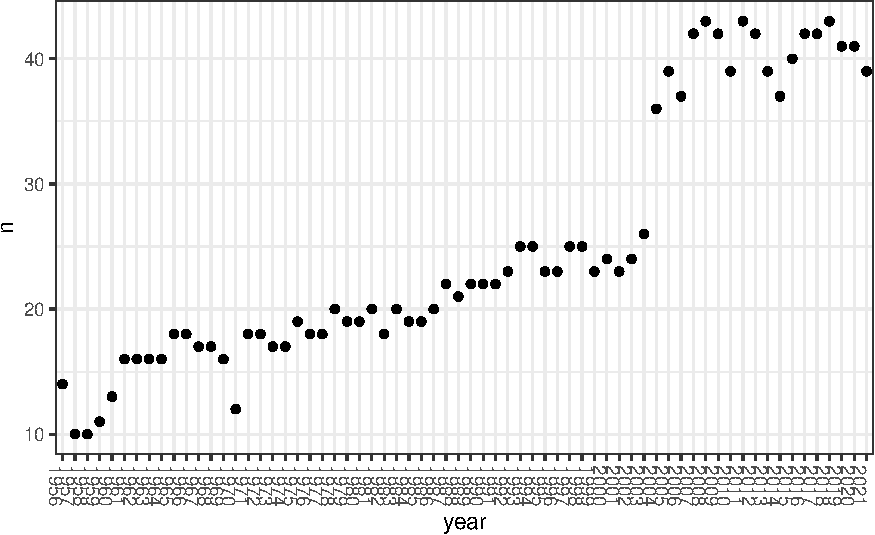
\includegraphics[width=0.7\linewidth]{DS_CS02_Data_Cleaning_Eurovision_files/figure-latex/unnamed-chunk-12-1} \end{center}

\subsection{Lyrics}\label{lyrics}

\begin{Shaded}
\begin{Highlighting}[]
\NormalTok{songs }\SpecialCharTok{\%\textgreater{}\%} 
  \FunctionTok{sample\_n}\NormalTok{(}\DecValTok{5}\NormalTok{) }\SpecialCharTok{\%\textgreater{}\%} 
  \FunctionTok{pull}\NormalTok{(lyrics) }\SpecialCharTok{\%\textgreater{}\%} 
  \FunctionTok{cat}\NormalTok{(}\AttributeTok{sep =} \StringTok{"}\SpecialCharTok{\textbackslash{}n\textbackslash{}n\textbackslash{}n}\StringTok{"}\NormalTok{)}
\end{Highlighting}
\end{Shaded}

\begin{verbatim}
## It's been a long time since we were together
## I'm back in Ireland and I miss you more than ever
## In early spring we parted and I've been here since then
## But if I could only see you once again
## 
## Meet me in Paris on a Champs-Élysées night
## We could be in Rome again, 'neath the Trevi fountain light
## We should be together, and maybe we just might
## If you could only meet me somewhere in Europe tonight
## 
## I remember Amsterdam as we sailed along the canal
## And as the leaves began to fall, we were walking in old Bruxelles
## In the Black Forest on a German summer's day
## And the memories refuse to go away
## 
## Meet me in Paris on a Champs-Élysées night
## We could be in Rome again, 'neath the Trevi fountain light
## We should be together, and maybe we just might
## If you could only meet me somewhere in Europe
## 
## Don't you remember those Adriatic days?
## I miss your laughter and all your little ways
## I can still see you in London, walking on Trafalgar Square
## And drinking wine in Old Seville, how I wish that we were there
## 
## Meet me in Paris on a Champs-Élysées night
## We could be in Rome again, 'neath the Trevi fountain light
## We should be together, maybe we just might
## If you could only meet me somewhere in Europe tonight
## 
## Meet me in Paris on a Champs-Élysées night
## We could be in Rome again, 'neath the Trevi fountain light
## We should be together, and maybe we just might
## If you could only meet me somewhere in Europe tonight
## 
## Somewhere in Europe tonight
## Somewhere in Europe
## 
## 
## Pam padadam padadam...
## Padada dadadam...
## Padadam padadam...
## 
## À l'horizon, une touche d'argent
## Comme après l'orage, s'en vont les nuages
## Les nuits d'été, sommeil oublié
## Grâce à ton parfum, je retrouve mon chemin
## 
## Il pleut de l'or, chaque fois que tu me parles d'amour
## Il pleut de l'or, ensemble partons pour faire le grand tour
## Sous la voûte étoilée, les destins sont dorés
## Il pleut de l'or
## 
## Pam padadam padadam...
## Padada dadadam...
## Padadam padadam...
## 
## Et au matin, secrets communs
## Les regards échangés sont complices de l'été
## Le jour chasse la magie
## Reste les yeux qui brillent
## 
## Il pleut de l'or, chaque fois que tu me parles d'amour (Il pleut de l'or)
## Il pleut de l'or, ensemble partons pour faire le grand tour
## Sous la voûte étoilée, les destins sont dorés
## Il pleut de l'or, toute la nuit et jusqu'à l'aurore
## Il pleut de l'or
## 
## Danse avec moi, vole avec moi
## Parle tout bas, parle-moi
## 
## (Il pleut de l'or) Il pleut de l'or
## (Il pleut de l'or)
## 
## Il pleut de l'or, ensemble partons pour faire le grand tour
## Sous la voûte étoilée, les destins sont dorés
## Il pleut de l'or, toute la nuit et jusqu'à l'aurore
## Il pleut de l'or
## 
## 
## spoken:
## "Και γαρ εβούλοντο μυάναι την γην ταύτην
## Μη γιγνώσκοντες την ύβριν, ην εποίουν..."
## 
## Είχα μια περιουσία, την καταχραστήκανε
## Κάναν ιεροσυλία κι ούτε που ντραπήκανε
## Την ιστορία της ζωής μου δε σκεφτήκανε
## 
## Ποια προσευχή εγώ να κάνω για τα κρίματά τους
## Ποια προσευχή μπορώ να πω για να σωθούν
## Στάζω κρασί για να ξεπλύνω τ' αμαρτήματά τους
## Ποια προσευχή να πω γι' αυτούς, που με πονούν
## 
## Να μου πάρουνε το θρόνο κάποιοι προσπαθήσανε
## Έν' αστέρι είχα μόνο και το απαιτήσανε
## Το πόσο άντεξα στο χρόνο αγνοήσανε
## 
## Ποια προσευχή εγώ να κάνω για τα κρίματά τους
## Ποια προσευχή μπορώ να πω για να σωθούν
## Στάζω κρασί για να ξεπλύνω τ' αμαρτήματά τους
## Ποια προσευχή να πω γι' αυτούς, που με πονούν
## 
## Ποια προσευχή εγώ να κάνω για τα κρίματά τους
## Ποια προσευχή μπορώ να πω για να σωθούν
## Στάζω κρασί για να ξεπλύνω τ' αμαρτήματά τους
## Ποια προσευχή να πω γι' αυτούς, που με πονούν
## 
## 
## [Verse 1: Jessika]
## Bullied from the moment we were born
## We were always on our own
## No one ever said we should be proud
## Or embrace the fact of standing out
## Forward too long, we just played along
## Always putting up a show
## But that was then, look at us now
## All we want is for them to know
## 
## [Pre-Chorus 1: Jessika]
## We are who we are
## And who we are is who we wanna be
## We don't have to listen
## 'Cause all that counts is you and me
## 
## [Chorus 1: Jessika]
## And then we’ll be rising where we fall, oh, oh
## In the middle of storm we're standing tall, oh, standing tall
## And if they tell us why we're wrong, oh, oh
## Then the love in our hearts will keep us strong, oh, oh
## 
## [Verse 2: Jenifer Brening]
## Uh listen up. listen up
## It's me, Jenny B, what you get is what you see
## As for Jess over here, she's a special VIP
## So you better listen carefully
## If they dissin' you on Twitter
## Don't get sad, don't be bitter, don't give up or be a quitter
## Show them you're better (yeah, hell no)
## If they say so, get in the car, rev it up, and be it a star
## 'Cause you know who exactly who we are
## Give it to 'em, Jess
## 
## [Pre-Chorus 2: Jessika & Jenifer Brening]
## We are who we are (yeah)
## And who we are is who we wanna be
## We don't have to listen (don't listen)
## 'Cause all that counts is you and me (hey, hey, hey, hey)
## 
## [Chorus 2: Jessika & Jenifer Brening]
## And then we’ll be rising where we fall, oh, oh yeah, we keep getting up and dusting ourselves off
## In the middle of storm we're standing tall (we won’t doubt ourselves and we’ll be calling their bluff)
## Oh, standing tall (this is who we are)
## And if they tell us why we're wrong, oh, oh (we will march onward, spreading the love)
## Then the love in our hearts will keep us strong, oh, oh (yeah, yeah, yeah)
## 
## [Bridge: Jessika]
## They can make it silent
## But in our hearts we'll never be
## 
## [Outro: Jessika & Jenifer Brening]
## And then we’ll be rising where we fall, oh, yeah (yeah, yeah)
## In the middle of storm we're standing tall, oh, standing tall
## And if they tell us why we're wrong, oh, oh, yeah
## Then the love in our hearts will keep us strong, oh, oh
## 
## 
## (M. Fabrizio/R. Fogli/V. Spampinato)
## Buonasera quando arriverai
## Ti toglierai l'inverno e lo appenderai
## Avrai due braccia grandi come una foresta
## E la quiete dopo la tempesta
## 
## Per Lucia, ritrovare
## Il foglio più bianco e poi cominciare;
## Io vorrei, per esempio
## Legarle i capelli con un filo di vento;
## Per Lucia basta poco
## Ti riempie da sola il giorno più vuoto;
## Io vorrei così tanto
## Ridarle il sorriso, sul viso un po' stanco
## 
## Oltre il muro, che cosa c'è
## Trattieni il fiato e poi salta verso me;
## I colpi di fucile sono ormai lontani
## Apriremo il cielo con le mani
## 
## Per Lucia, lunga vita
## E acqua di fiume per ogni ferita;
## Io vorrei luci accese
## La festa più grande per tutto il paese;
## Per Lucia, spaventata
## Che questa mia penna diventi una spada;
## Con Lucia al mio fianco
## Che la storia continui nella pagina accanto
\end{verbatim}

\subsection{Translation}\label{translation}

\begin{Shaded}
\begin{Highlighting}[]
\NormalTok{songs }\SpecialCharTok{\%\textgreater{}\%} 
  \FunctionTok{sample\_n}\NormalTok{(}\DecValTok{5}\NormalTok{) }\SpecialCharTok{\%\textgreater{}\%} 
  \FunctionTok{pull}\NormalTok{(translation) }\SpecialCharTok{\%\textgreater{}\%} 
  \FunctionTok{cat}\NormalTok{(}\AttributeTok{sep =} \StringTok{"}\SpecialCharTok{\textbackslash{}n\textbackslash{}n\textbackslash{}n}\StringTok{"}\NormalTok{)}
\end{Highlighting}
\end{Shaded}

\begin{verbatim}
## When there is nothing else, I think that
## I still have a song I can sing to you
## About happiness we feel, about a road that goes
## Like a train on metal rails To faraway stations on the North Pole
## Where freedom lives, and nothing else
## Each time when I feel miracles in the distance
## I want to be closer to you Nothing, when there is nothing else
## I want to sing you a song about happiness
## That comes, that comes unexpectedly
## And takes us by the hand
## A song about happiness to come When there is nothing else, I think that
## I still have the wind that runs up to the sky
## And the sun that rises, faraway roads that cross
## Seven mountains and nine seas To warmer lands like birds of passage
## There everything is just like in a dream, but you are not there
## Each time when I feel miracles in the distance
## I want to be closer to you Nothing, when there is nothing else
## I want to sing you a song about happiness
## That comes, that comes unexpectedly
## And takes us by the hand
## A song about happiness to come Nothing, when there is nothing else
## I want to sing you a song about happiness
## That comes, that comes unexpectedly
## And takes us by the hand
## A song about happiness to come Nothing, when there is nothing else
## I want to sing you a song about happiness
## That comes, that comes unexpectedly
## And takes us by the hand
## A song to come
## A song about happiness to come
## 
## 
## English
## 
## 
## English
## 
## 
## English
## 
## 
## Sometimes, words are unnecessary
## When it's about talking
## Simply of love
## And I prefer the eloquence of a silence
## To that weary phrase
## That sounds like nothing in my voice. I know that you can believe
## That I lack the interest
## But sometimes the most fervent promises
## Only try to hide that love is dying. Love, love, my love
## You'd have to accept me this way
## If you see that I don't like to talk
## Learn to understand my absence. Love, love, my love
## It's all I can say
## To love is something more than making laugh
## I know I'll fill your life with love.
\end{verbatim}

\subsection{Place}\label{place}

\begin{Shaded}
\begin{Highlighting}[]
\NormalTok{songs }\SpecialCharTok{\%\textgreater{}\%} \FunctionTok{count}\NormalTok{(place)}
\end{Highlighting}
\end{Shaded}

\begin{verbatim}
## # A tibble: 27 x 2
##    place     n
##    <chr> <int>
##  1 -       309
##  2 1        68
##  3 10       66
##  4 11       58
##  5 12       60
##  6 13       70
##  7 14       59
##  8 15       53
##  9 16       56
## 10 17       48
## # i 17 more rows
\end{verbatim}

\begin{Shaded}
\begin{Highlighting}[]
\FunctionTok{length}\NormalTok{(}\FunctionTok{unique}\NormalTok{(songs}\SpecialCharTok{$}\NormalTok{year))}
\end{Highlighting}
\end{Shaded}

\begin{verbatim}
## [1] 66
\end{verbatim}

\begin{Shaded}
\begin{Highlighting}[]
\NormalTok{songs }\SpecialCharTok{\%\textgreater{}\%} 
  \FunctionTok{count}\NormalTok{(year, place) }\SpecialCharTok{\%\textgreater{}\%} 
  \FunctionTok{filter}\NormalTok{(place }\SpecialCharTok{==} \StringTok{"1"}\NormalTok{) }\SpecialCharTok{\%\textgreater{}\%} 
  \FunctionTok{arrange}\NormalTok{(}\SpecialCharTok{{-}}\NormalTok{n)}
\end{Highlighting}
\end{Shaded}

\begin{verbatim}
## # A tibble: 65 x 3
##    year  place     n
##    <chr> <chr> <int>
##  1 1969  1         4
##  2 1956  1         1
##  3 1957  1         1
##  4 1958  1         1
##  5 1959  1         1
##  6 1960  1         1
##  7 1961  1         1
##  8 1962  1         1
##  9 1963  1         1
## 10 1964  1         1
## # i 55 more rows
\end{verbatim}

According to Wikpedia, there were four winners in 1969:

\url{https://en.wikipedia.org/wiki/Eurovision_Song_Contest}

\begin{quote}
On only one occasion have multiple winners been declared in a single
contest: in 1969, four countries finished the contest with an equal
number of votes and due to the lack of a tie-break rule at the time, all
four countries were declared winners.{[}7{]}{[}157{]}
\end{quote}

\section{Rule 6: You May Need to Go
Back}\label{rule-6-you-may-need-to-go-back}

Our original parse function just grabbed \texttt{translation} as is.
After looking at \texttt{translation}, we can see that this variable
says \texttt{English} if the original song lyrics are in English.
English.

\section{Rule 7: Create New Columns?}\label{rule-7-create-new-columns}

\subsection{Decade}\label{decade}

\begin{Shaded}
\begin{Highlighting}[]
\NormalTok{songs}
\end{Highlighting}
\end{Shaded}

\begin{verbatim}
## # A tibble: 1,644 x 7
##    country        artist                 title    year  lyrics translation place
##    <chr>          <chr>                  <chr>    <chr> <chr>  <chr>       <chr>
##  1 Netherlands    Jetty Paerl            De voge~ 1956  "De v~ "The birds~ -    
##  2 Switzerland    Lys Assia              Das alt~ 1956  "Das ~ "The old c~ -    
##  3 Belgium        Fud Leclerc            Messieu~ 1956  "Mess~ "Ye drowne~ -    
##  4 Germany (West) Walter Andreas Schwarz Im Wart~ 1956  "Es g~ "There is ~ -    
##  5 France         Mathé Altéry           Le temp~ 1956  "Chan~ "Sing, car~ -    
##  6 Luxembourg     Michèle Arnaud         Ne croi~ 1956  "Si o~ "If they t~ -    
##  7 Italy          Franca Raimondi        Aprite ~ 1956  "La p~ "The first~ -    
##  8 Netherlands    Corry Brokken          Voorgoe~ 1956  "Voor~ "Over for ~ -    
##  9 Switzerland    Lys Assia (2)          Refrain  1956  "[Int~ "Chorus of~ 1    
## 10 Belgium        Mony Marc              Le plus~ 1956  "Les ~ "The bells~ -    
## # i 1,634 more rows
\end{verbatim}

\begin{Shaded}
\begin{Highlighting}[]
\NormalTok{songs }\OtherTok{\textless{}{-}} 
\NormalTok{  songs }\SpecialCharTok{\%\textgreater{}\%} 
  \FunctionTok{mutate}\NormalTok{(}
    \AttributeTok{year =} \FunctionTok{parse\_number}\NormalTok{(year), }
    \AttributeTok{decade =}\NormalTok{ year }\SpecialCharTok{{-}}\NormalTok{ year }\SpecialCharTok{\%\%} \DecValTok{10}
\NormalTok{  )}
\NormalTok{songs }\SpecialCharTok{\%\textgreater{}\%} 
  \FunctionTok{ggplot}\NormalTok{(}\FunctionTok{aes}\NormalTok{(year, decade)) }\SpecialCharTok{+} 
  \FunctionTok{geom\_point}\NormalTok{()}
\end{Highlighting}
\end{Shaded}

\begin{center}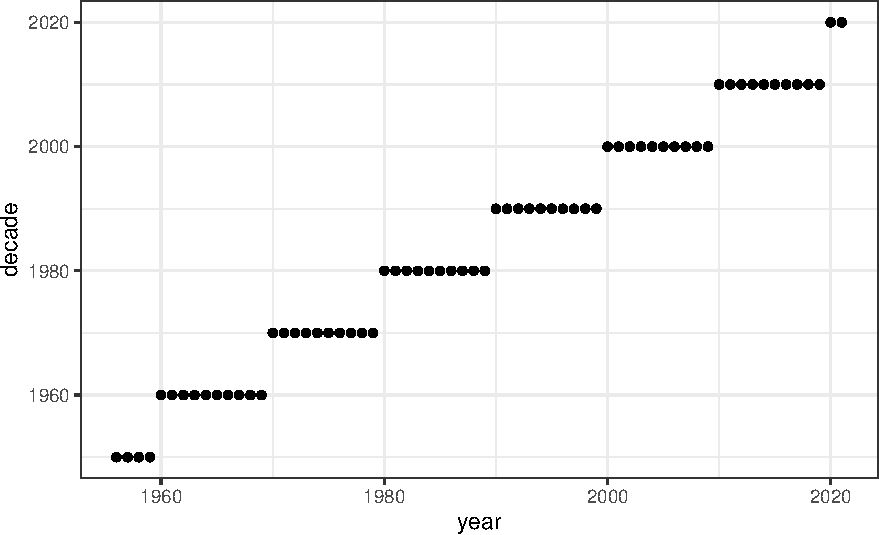
\includegraphics[width=0.7\linewidth]{DS_CS02_Data_Cleaning_Eurovision_files/figure-latex/unnamed-chunk-18-1} \end{center}

\subsection{Lyrics}\label{lyrics-1}

\begin{Shaded}
\begin{Highlighting}[]
\NormalTok{songs }\SpecialCharTok{\%\textgreater{}\%} 
  \FunctionTok{count}\NormalTok{(translation) }\SpecialCharTok{\%\textgreater{}\%}
  \FunctionTok{arrange}\NormalTok{(}\SpecialCharTok{{-}}\NormalTok{n)}
\end{Highlighting}
\end{Shaded}

\begin{verbatim}
## # A tibble: 946 x 2
##    translation                                                                 n
##    <chr>                                                                   <int>
##  1 "English"                                                                 694
##  2 ""                                                                          2
##  3 "Day is turning to evening, is gone, soon forgotten\nBut what we gave ~     2
##  4 "God, god, god, god they don’t call you\nCandles, candles, candles, ca~     2
##  5 "Look into my eyes now,\nI'm not a looser, know it!\nI don't surrender~     2
##  6 "Only champions!\nOnly champions! They fly high1 and jump far2.\nAll t~     2
##  7 "\nPure and white, her skin is so inviting\nLike a new, unbeaten snow\~     1
##  8 "\"Come with me\", said my friend\nThe first silent winter snow is fal~     1
##  9 "\"This is the Telephone Information Service, hello\"\n\"Yes, hello, t~     1
## 10 "\"We are all moving around the old circle\"1,\nSinging in this sweet ~     1
## # i 936 more rows
\end{verbatim}

\begin{Shaded}
\begin{Highlighting}[]
\NormalTok{songs }\OtherTok{\textless{}{-}} 
\NormalTok{  songs }\SpecialCharTok{\%\textgreater{}\%} 
  \FunctionTok{mutate}\NormalTok{(}
    \AttributeTok{english\_lyrics =} \FunctionTok{ifelse}\NormalTok{(}
\NormalTok{      translation }\SpecialCharTok{==} \StringTok{"English"}\NormalTok{,}
\NormalTok{      lyrics, translation}
\NormalTok{    ) }
\NormalTok{  )}
\end{Highlighting}
\end{Shaded}

\section{Rule 7: Save the Data and Write it
Up}\label{rule-7-save-the-data-and-write-it-up}

It's critically important to make detailed notes about any changes you
have made when cleaning the data.

\begin{Shaded}
\begin{Highlighting}[]
\NormalTok{filenamepath }\OtherTok{\textless{}{-}}\NormalTok{ glue}\SpecialCharTok{::}\FunctionTok{glue}\NormalTok{(}\StringTok{"./data/\{lubridate::today()\}{-}eurovision.rds"}\NormalTok{)}
\NormalTok{filenamepath}
\end{Highlighting}
\end{Shaded}

\begin{verbatim}
## ./data/2025-02-17-eurovision.rds
\end{verbatim}

\begin{Shaded}
\begin{Highlighting}[]
\FunctionTok{write\_rds}\NormalTok{(songs,filenamepath)}
\end{Highlighting}
\end{Shaded}


\end{document}
